\documentclass[a4paper, 12pt]{report}

%%%%%%%%%%%%
% Packages %
%%%%%%%%%%%%

\usepackage[english]{babel}
\usepackage[noheader]{packages/sleek}
\usepackage{packages/sleek-title}
\usepackage{packages/sleek-theorems}
\usepackage{packages/sleek-listings}
\usepackage{amsmath}
\usepackage[normalem]{ulem}
\useunder{\uline}{\ul}{}
\usepackage{comment}
\usepackage{hyperref}
\usepackage{listings}
\lstset{language=Python}
\lstset{frame=lines}
\lstset{basicstyle=\footnotesize}
\usepackage{multirow}
\setcounter{tocdepth}{3}
\setcounter{secnumdepth}{3}
\graphicspath{ {figures/} }
\usepackage{array}
\definecolor{mygreen}{rgb}{0,0.6,0}
\definecolor{mygray}{rgb}{0.5,0.5,0.5}
\definecolor{mymauve}{rgb}{0.58,0,0.82}
\definecolor{myorange}{rgb}{0.855,0.576,0.027}

%%%%%%%%%%%%%%
% Title-page %
%%%%%%%%%%%%%%

\logo{./resources/pdf/logo.pdf}
\institute{Department Of Aerospace Engineering}
\faculty{AS2101\\Prof. Bharath Govindarajan\\Prof. Ramakrishna M }
\title{NUMERICAL COMPUTATION OF A UNIVARIATE DEFINITE INTEGRAL\\TASK 4: 31-07-2021(Due-Date) }
\subtitle{REPORT}
\author{\textbf{AUTHOR}\\Yash Singh Jha-(AE19B016)\\ }

 \date{July 31 , 2021}


%%%%%%%%%%%%%%%%
% Bibliography %
%%%%%%%%%%%%%%%%

\addbibresource{./resources/bib/references.bib}

%%%%%%%%%%
% Others %
%%%%%%%%%%

\lstdefinestyle{latex}{
    language=TeX,
    style=default,
    %%%%%
    commentstyle=\ForestGreen,
    keywordstyle=\TrueBlue,
    stringstyle=\VeronicaPurple,
    emphstyle=\TrueBlue,
    %%%%%
    emph={LaTeX, usepackage, textit, textbf, textsc}
}

\FrameTBStyle{latex}

\def\tbs{\textbackslash}

%%%%%%%%%%%%
% Document %
%%%%%%%%%%%%

\begin{document}
    \maketitle
    \romantableofcontents
    \listoffigures
    \begin{abstract}
    This document is like a summary report of the work we were assigned as Task 4 in the course-AS2101.\\
    This report presents a few of the various methods/algorithms used to calculate the numerical integral of a definite integral of a univariate function. We discuss two main methods - \textbf{Rectangular Method} and \textbf{Trapezoidal Method}. Three submethods of the Rectangular Method - Left Endpoint, Right Endpoint and the Midpoint Methods, are also discussed. \\
    Chapter 1 - \textbf{Numerical Quadrature}, deals with the theory behind each of the above mentioned methods and illustrates the philosophy behind it elegantly using appropriate equations and figures. It also explains the theory behind absolute error and order of accuracy of each of these methods.\\
    Chapter 2 - \textbf{Numerical Computation : Python Implementation}, presents and discusses the methods in Python -  their characteristics and differences.\\
    Chapter 3 - \textbf{Results}, takes us through the results obtained using the Python codes presented in chapter 2 and compares the computational differences between them.\\
    Chapter 4 - \textbf{Conclusion}, presents a concluding remark on the overall report and the materials covered. It also gives a comment on the relative accuracy/usage of the methods.\\
    This LaTeX file itself is the part of the task for the third week of AS2101.
    \end{abstract}
    
    \chapter{Numerical Quadrature}
In analysis, numerical integration comprises a broad family of algorithms for calculating the numerical value of a definite integral, and by extension, the term is also sometimes used to describe the numerical solution of differential equations. This report focuses on calculation of definite integrals of univariate functions. Refer figure~\ref{fig:NumInt}.\\
 \begin{figure}[h]
    \centering
    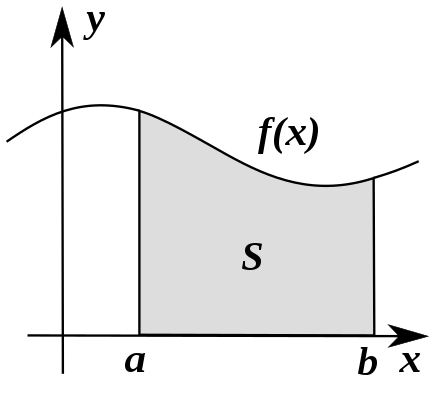
\includegraphics[width=10cm]{NumInt.png}
    \caption{Numerical integration is used to calculate a numerical approximation for the value \textbf{S}, the area under the curve defined by \textbf{f(x)}.}
    \label{fig:NumInt}
    \end{figure}
The term numerical quadrature (often abbreviated to quadrature) is more or less a synonym for numerical integration, especially as applied to one-dimensional integrals. Some authors refer to numerical integration over more than one dimension as cubature; others take quadrature to include higher-dimensional integration.\\
The basic problem in numerical integration is to compute an approximate solution to a definite integral
\begin{equation}
    \int_{a}^{b} f(x)\,dx\
\label{eqn1}
\end{equation}
to a given degree of accuracy. If $f(x)$ is a smooth function integrated over a small number of dimensions, and the domain of integration is bounded, there are many methods for approximating the integral to the desired precision.
    \section{Reasons for Numerical Integration}
   There are several reasons for carrying out numerical integration, as opposed to analytical integration by finding the antiderivative:
   \begin{enumerate}
       \item The integrand $f(x)$ may be known only at certain points, such as obtained by sampling. Some embedded systems and other computer applications may need numerical integration for this reason.
       \item A formula for the integrand may be known, but it may be difficult or impossible to find an antiderivative that is an elementary function. An example of such an integrand is $f(x) = e^{-x^{2}}$, the antiderivative of which (the error function, times a constant) cannot be written in elementary form.
       \item It may be possible to find an antiderivative symbolically, but it may be easier to compute a numerical approximation than to compute the antiderivative. That may be the case if the antiderivative is given as an infinite series or product, or if its evaluation requires a special function that is not available.
   \end{enumerate}
    \section{Rectangle Method}
    Here, we wish to approximate a definite integral \ref{eqn1} where $f(x)$ is a continuous function. \\
    We begin by choosing points{$x_{i}$} that subdivide $[a,b]$:
    \begin{equation}
        a = x_{0}<x_{1}<.....<x_{n-1}<x_{n} = b
    \end{equation}
    The subintervals $[x_{i-1},x_{i}]$ determine the width $\Delta x_{i}$ of each of the approximating rectangles. For height, we can choose any value $f(x*)$, where x* $\epsilon$ $[x_{i-1},x_{i}]$. the resulting approximation is 
    \begin{equation}
         \int_{a}^{b} f(x)\,dx\  \approx \Sigma_{i=1}^{n} f(x*_{i}) \Delta x_{i}
    \end{equation}
    To use this to approximate integrals with actual numbers, we need to have a specific $x*_{i}$ in each interval. The two simplest (and relatively erroneous) ways to choose $x*_{i}$ are as the left-hand point or the right-hand point of the each subinterval. This gives concrete approximations -Left Riemann Sum and Right Riemann Sum, which we denote by $L_{n}$ and $R_{n}$ given by 
    \begin{equation}
        L_{n} = \Sigma_{i=1}^{n} f(x_{i-1}) \Delta x_{i}
    \end{equation}
    and 
     \begin{equation}
        R_{n} = \Sigma_{i=1}^{n} f(x_{i}) \Delta x_{i}
    \end{equation}
    To keep things from getting too messy, we choose our subintervals of equal length i.e $\Delta x_{i} = \Delta x$. The approximations become better as the number of subintervals increase.
    \subsection{Left-Endpoint Method}
    For the left Riemann sum, approximating the function by its value at the left-end point gives multiple rectangles with base $\Delta x$ and height $f(a+i\Delta x)$. Doing this for $i = 0,1,...,n-1$ and adding up the resultant areas gives
    \begin{equation}
        L_{n} = \Delta x[f(a) + f(a+\Delta x) + f(a+2\Delta x) + ...+ f(b-\Delta x)]
    \end{equation}
    \begin{figure}[h]
    \centering
    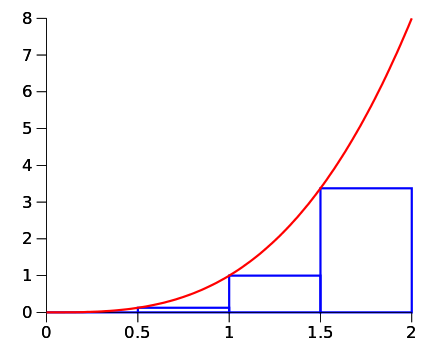
\includegraphics[width=10cm]{LeftRS.png}
    \caption{Left Riemann sum of $x^{3}$ over [0,2] using 4 subdivisions}
    \label{fig:LeftRS}
    \end{figure}
    The left Riemann sum amounts to an overestimation if $f$ is monotonically decreasing on this interval, and an underestimation if it is monotonically increasing. Refer \ref{fig:LeftRS}.
    \subsection{Right-Endpoint Method}
    For the right Riemann sum, approximating the function by its value at the right-end point gives multiple rectangles with base $\Delta x$ and height $f(a+i\Delta x)$. Doing this for $i = 0,1,...,n-1$ and adding up the resultant areas gives
    \begin{equation}
        R_{n} = \Delta x[f(a+\Delta x) +  f(a+2\Delta x) + ...+ f(b)]
    \end{equation}
    \begin{figure}[!h]
    \centering
    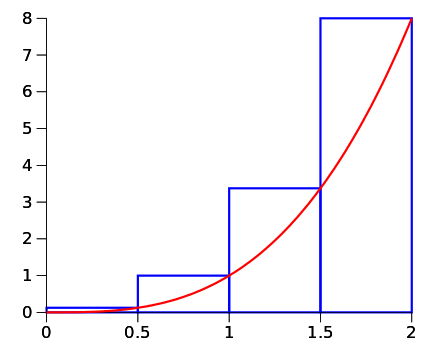
\includegraphics[width=10cm]{RightRS.png}
    \caption{Right Riemann sum of $x^{3}$ over [0,2] using 4 subdivisions}
    \label{fig:RightRS}
    \end{figure}
    The right Riemann sum amounts to an overestimation if $f$ is monotonically increasing on this interval, and an underestimation if it is monotonically decreasing.Refer \ref{fig:RightRS}.\\
    The error of this formula will be 
    \begin{equation}
        \abs{ \int_{a}^{b} f(x)\,dx\  - R_{n}} \leq \frac{M_{1}(b-a)^{2}}{2n}
    \end{equation}
    where $M_{1}$ is the maximum value of $\abs{f'(x)}$ on the interval.
    \subsection{Midpoint Method}
    \begin{figure}[!h]
    \centering
    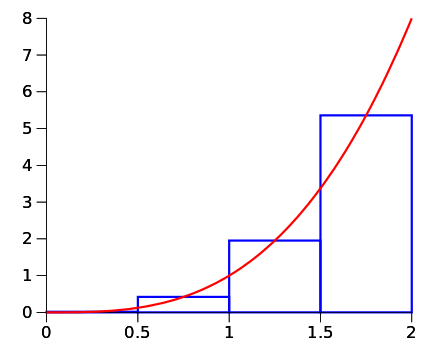
\includegraphics[width=10cm]{MidRS.png}
    \caption{Midpoint Riemann sum of $x^{3}$ over [0,2] using 4 subdivisions}
    \label{fig:MidRS}
    \end{figure}
    Approximating $f$ at the midpoint of the intervals gives $f(a+\Delta x /2)$ for the first interval, for the next one $f(a+3\Delta x /2)$, and so on until $f(b-\Delta x /2)$.Refer \ref{fig:MidRS}. Summing up the areas gives
    \begin{equation}
        M_{n} = \Delta x[f(a+\frac{1}{2}\Delta x ) +  f(a+\frac{3}{2}\Delta x ) + ...+ f(b-\frac{1}{2}\Delta)]
    \end{equation}
    The error of this formula will be
     \begin{equation}
        \abs{ \int_{a}^{b} f(x)\,dx\  - M_{n}} \leq \frac{M_{2}(b-a)^{3}}{24n^{2}}
    \end{equation}
    where $M_{2}$ is the maximum value of the absolute value of $f''(x)$ on the interval.
   
    \subsection{Example: Using Left, Right and Midpoint rules.}
    In this subsection, we explain the usage of Left, Right and Midpoint Rules by approximating the area under $f(x)=4x-x^{2}$ on the interval $[0,4]$ using each of the methods, using 4 equally spaced intervals.\\
    In figure \ref{fig:EL}, we see four rectangles drawn on $f(x)=4x-x^{2}$ using the Left Hand Rule. (The areas of the rectangles are given in each figure.)
    \begin{figure}[h]
    \centering
    \begin{subfigure}{.55\textwidth}
    \centering
    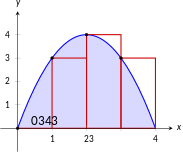
\includegraphics[width=.95\linewidth]{EL.png}
    \caption{Left Hand Rule.}
    \label{fig:EL}
    \end{subfigure}%    
    \begin{subfigure}{.55\textwidth}
    \centering
    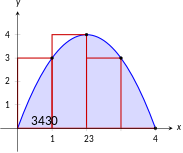
\includegraphics[width=.95\linewidth]{ER.png}
    \caption{Right Hand Rule}
    \label{fig:ER}
    \end{subfigure}
    \begin{subfigure}{.6\textwidth}
    \centering
    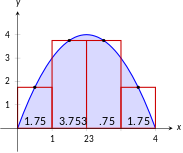
\includegraphics[width=.95\linewidth]{EM.png}
    \caption{Midpoint Rule}
    \label{fig:EM}
    \end{subfigure}
    \end{figure}
    Note, how in the first subinterval [0,1], the rectangle has height $f(0)=0$. We add up the areas of each rectangle for our Left Hand Rule approximation:
    \begin{equation}
        f(0).1 + f(1).1 + f(2).1 + f(3).1 = 0 + 3 + 4 + 3 = 10
    \end{equation}
    Figure \ref{fig:ER}, shows 4 rectangles drawn under $f(x)$ using the Right Hand Rule; note how the [3,4] subinterval has a rectangle of height 0.
    In this figure, these rectangles seem to be the mirror image of those found in figure \ref{fig:EL}. (This is because of the symmetry of our shaded region.). Our approximation gives the same answer as before, though calculated a different way:
    \begin{equation}
        f(1).1 + f(2).1 + f(3).1 + f(4).1 =  3 + 4 + 3 + 0 = 10
    \end{equation}
    Figure \ref{fig:EM}, shows 4 rectangles drawn under $f(x)$ using the Midpoint Rule.
    This gives an approximation of the area as :
    \begin{equation}
        f(0.5).1 + f(1.5).1 + f(2.5).1 + f(3.5).1 =  1.75 + 3.75 + 3.75 + 1.75 = 11
    \end{equation}
    Our three methods provide two approximations of the area under \textbf{$f(x)=4x-x^{2}$}: \textbf{10} and \textbf{11}.
    
    \section{Trapezoid Method}
     \begin{figure}[!h]
    \centering
    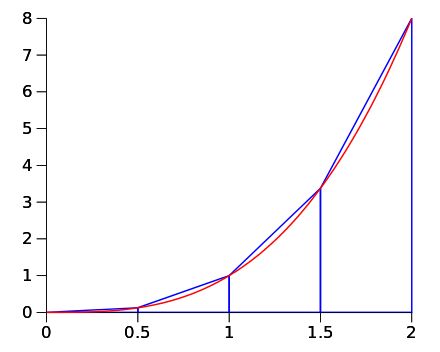
\includegraphics[width=10cm]{TrapRS.png}
    \caption{Trapezoidal Riemann sum of $x^{3}$ over [0,2] using 4 subdivisions}
    \label{fig:TrapRS}
    \end{figure}
    In this case, the values of the function $f$ on an interval are approximated by the average of the values at the left and right endpoints.Refer figure~\ref{fig:TrapRS} In the same manner as above, a simple calculation using the area formula
    \begin{equation}
        A = \frac{h(b_{1}+b_{2})}{2}
    \end{equation}
    for a trapezium with parallel sides $b_{1}$, $b_{2}$ and height h produces
     \begin{equation}
        A_{trap} = \frac{1}{2}\Delta x[f(a) + 2f(a+\Delta x ) + 2f(a+2\Delta x ) ...+ f(b)]
    \end{equation}
    The error of this formula will be
     \begin{equation}
        \abs{ \int_{a}^{b} f(x)\,dx\  - A_{trap}} \leq \frac{M_{2}(b-a)^{3}}{12n^{2}}
    \end{equation}
    where $M_{2}$ is the maximum value of the $\abs{f''(x)}$.\\
    The approximation obtained with the trapezoid rule for a function is the same as the average of the left hand and right hand sums of that function.
   
    \section{Absolute Error}
    An important aspect of using these numerical approximation rules consists of calculating error in using them for estimating the value of a definite integral. We first need to define absolute error and relative error.\\
    \textbf{Absolute Error: $\abs{E}$} If $B$ is our estimation of some quantity having an actual value of $A$, then the absolute error is given by $\abs{A-B}$.\\
    \textbf{Relative Error:} The relative error is the error as a percentage of the actual value and is given by 
    \begin{equation}
        \abs{\frac{A-B}{A}}.100\%
    \end{equation}
    Evaluating $f$ at many points may be computationally expensive, or difficult for other reasons, e.g if $f$ is given by measurements. It is therefore important to consider how the error $E$ depends on n. Obviously, one would expect $E$ to become small as n becomes large. In a set of measurements, accuracy is closeness of the measurements to a specific value. So, even by logic the consideration of order of accuracy in our analysis/results is very important. We define it as follows.\\
    \textbf{Order of Accuracy:} It shows how fast $\abs{E}$ decays to zero when we take a smaller distance $h$ between the nodes. Since, $n\approx \frac{1}{h}$ in these rules (at least in 1D), it similarly describes how fast $E\to 0$ when $n \to \inf$. We define the order of accuracy as the largest number p for which there exists a constant $C$, independent of $h$ for which 
    \begin{equation}
        \abs{E} \leq C h^{p}
    \end{equation}
    For our report,
    \begin{equation}
        \abs{E} = \abs{\int_{0}^{\pi/2}\sin{x}\,dx\ - e}
    \end{equation}
    Further comments on accuracy and order of accuracy are provided later in the report.
 \chapter{ Numerical Computation : Python Implementation}
This chapter takes us through the codes in Python used to implement the theory provided to us in the preceding chapter or in other words - here, we go through the Python Code for the numerical implementation of the Rectangle Method (Left, Right and Midpoint methods) and the Trapezoid Method.
\section{Rectangle Method}
The following code in Python, is the implementation of the theory and iteration tasks covered in the previous chapters. The code is commented well so further explanation of the code doesn't seem necessary.Results of the code~\ref{lst:LM}, \ref{lst:RM} and \ref{lst:MpM} are presented in the next chapter, in plots  ~\ref{fig:Plot1}, \ref{fig:Plot2} and \ref{fig:Plot3} respectively.
\lstset{caption={Function named \textbf{'LM'} is constructed to carry out the numerical integration. }}
\lstset{label={lst:LM}}
\begin{lstlisting}
def LM(f,a,b,n):
    # Carries out the numerical integration using the Left Hand Rule
    # INPUT: f , a , b , n
    # f : function which is the integrand
    # a : lower limit of the interval
    # b : upper limit of the interval
    # n : number of sub-intervals

    # makes sure the input format is correct
    if (b < a) :
        print('Input Error: Lower limit(a) must be < Upper limit(b)')
        exit()
    # limits the maximum number of iterations to 1 million
    if (n > 1000000) :
        print('Input Error: No more than 1 million divisions are allowed!')
        exit()
    # calculate the step size or length of each sub-interval
    h = (b - a)/n
    # calculates the numerical integration using Left Hand Rule
    area = 0
    for i in range(n):
        x = a + float(i*h)
        area = area + f(x)*h
    # calculates error
    err = 1 - area
    rel_err = np.abs(err)*100
    print('---------------------------------------------------')
    print('NUMERICAL QUADRATURE RESULTS : LEFT-ENDPOINT METHOD')
    print('---------------------------------------------------')
    print('Integrating from %8.2f    to %8.2f   in %5d steps' %(a,b,n))
    print('Area           = %10.4f units\u00b2'%(area))
    print('Error          = %10.4f'%err)
    print('Absolute Error = %10.4f '%(np.abs(err)))
    print('Relative Error = %10.4f'%rel_err)
    print('---------------------------------------------------')
\end{lstlisting}

\lstset{caption={Function named \textbf{'RM'} is constructed to carry out the numerical integration. }}
\lstset{label={lst:RM}}
\begin{lstlisting}
def RM(f,a,b,n):
    # Carries out the numerical integration using the Right Hand Rule
    # INPUT: f , a , b , n
    # f : function which is the integrand
    # a : lower limit of the interval
    # b : upper limit of the interval
    # n : number of sub-intervals

    # makes sure the input format is correct
    if (b < a) :
        print('Input Error: Lower limit(a) must be < Upper limit(b)')
        exit()
    # limits the maximum number of iterations to 1 million
    if (n > 1000000) :
        print('Input Error: No more than 1 million divisions are allowed!')
        exit()
    # calculate the step size or length of each sub-interval
    h = (b - a)/n
    # calculates the numerical integration using Right Hand Rule
    area = 0
    for i in range(1,n+1):
        x = a + float(i*h)
        area = area + f(x)*h
    # calculates error
    err = 1 - area
    rel_err = np.abs(err)*100
    print('---------------------------------------------------')
    print('NUMERICAL QUADRATURE RESULTS : RIGHT-ENDPOINT METHOD')
    print('---------------------------------------------------')
    print('Integrating from %8.2f    to %8.2f   in %5d steps' %(a,b,n))
    print('Area           = %10.4f units\u00b2'%(area))
    print('Error          = %10.4f'%err)
    print('Absolute Error = %10.4f '%(np.abs(err)))
    print('Relative Error = %10.4f'%rel_err)
    print('---------------------------------------------------')
\end{lstlisting}
\lstset{caption={Function named \textbf{'MpM'} is constructed to carry out the numerical integration. }}
\lstset{label={lst:MpM}}
\begin{lstlisting}
def MpM(f,a,b,n):
    # Carries out the numerical integration using the Midpoint Rule
    # INPUT: f , a , b , n
    # f : function which is the integrand
    # a : lower limit of the interval
    # b : upper limit of the interval
    # n : number of sub-intervals

    # makes sure the input format is correct
    if (b < a) :
        print('Input Error: Lower limit(a) must be < Upper limit(b)')
        exit()
    # limits the maximum number of iterations to 1 million
    if (n > 1000000) :
        print('Input Error: No more than 1 million divisions are allowed!')
        exit()
    # calculate the step size or length of each sub-interval
    h = (b - a)/n
    # calculates the numerical integration using Midpoint Rule
    area = 0
    for i in range(n):
        x = a + float((i+0.5)*h)
        area = area + f(x)*h
    # calculates error
    err = 1 - area
    rel_err = np.abs(err)*100
    print('---------------------------------------------------')
    print('NUMERICAL QUADRATURE RESULTS : MIDPOINT METHOD')
    print('---------------------------------------------------')
    print('Integrating from %8.2f    to %8.2f   in %5d steps' %(a,b,n))
    print('Area           = %10.4f units\u00b2'%(area))
    print('Error          = %10.4f'%err)
    print('Absolute Error = %10.4f '%(np.abs(err)))
    print('Relative Error = %10.4f'%rel_err)
    print('---------------------------------------------------')
\end{lstlisting}
\section{Trapezoidal Method}
The task is repeated for Trapezoidal method here. For reference and better inference of the code, parallel viewing of the codes(\ref{lst:TM}) and the results(plot ~\ref{fig:Plot4}) provided in the next chapter is advised.
\lstset{caption={Function named \textbf{'TM'} is constructed to generate the iteration steps of the Newton's Method}}
\lstset{label={lst:TM}}
\begin{lstlisting}
def TM(f,a,b,n):
    # Carries out the numerical integration using the Trapezoidal Rule
    # INPUT: f , a , b , n
    # f : function which is the integrand
    # a : lower limit of the interval
    # b : upper limit of the interval
    # n : number of sub-intervals

    # makes sure the input format is correct
    if (b < a) :
        print('Input Error: Lower limit(a) must be < Upper limit(b)')
        exit()
    # limits the maximum number of iterations to 1 million
    if (n > 1000000) :
        print('Input Error: No more than 1 million divisions are allowed!')
        exit()
    # calculate the step size or length of each sub-interval
    h = (b - a)/n
    step.append(h)
    N.append(n)
    # calculates the numerical integration using Trapezoidal Rule
    area = f(float(a))*h/2
    for i in range(1,n):
        x = a + float(i*h)
        area = area + f(x)*h
    area = area + f(float(b))*h/2
    # calculates error
    err = 1 - area
    rel_err = np.abs(err)*100
    abs_err.append(np.abs(err))
    print('---------------------------------------------------')
    print('NUMERICAL QUADRATURE RESULTS : TRAPEZOID METHOD')
    print('---------------------------------------------------')
    print('Integrating from %8.2f    to %8.2f   in %5d steps' %(a,b,n))
    print('Area           = %10.4f units\u00b2'%(area))
    print('Error          = %10.4f'%err)
    print('Absolute Error = %10.4f '%(np.abs(err)))
    print('Relative Error = %10.4f'%rel_err)
    print('---------------------------------------------------')
\end{lstlisting}    
\section{Linear Regression of data.}
We were also required to plot (scatter) the raw data (Absolute Error and Step size/ number of intervals) obtained from the above codes and then use linear regression to plot a linear variation of the data, whose semi-log and log-log plots are also considered. Following code help carry out linear regression and plot them.
\lstset{caption={\textbf{inv() and linreg()}}}
\lstset{label={lst:linreg}}
\begin{lstlisting}
def inv(A):
    #Augment with an identity matrix of required order: Here it's 2 :
    if A.shape(0)!= A.shape(1):
       sys.exit('Not Invertible!')
    n = A.shape(0)
    a = np.concatenate((A,np.identity(n,dtype = float)),axis = 1)
    # Applying Gauss Jordan Elimination:
    for i in range(n):
        if a[i][i] == 0.0:
           sys.exit('Not Invertible!') 
        for j in range(n):
            if i != j:
               ratio = a[j][i]/a[i][i]
               for k in range(2*n):
                   a[j][k] = a[j][k] - ratio*a[i][k]
    #Row operation to make principal diagonal element to 1:
    for i in range(n):
        divisor = a[i][i]
        for j in range(2*n):
            a[i][j] = a[i][j]/divisor
    #Displaying the Inverted matrix:
    #print('\nINVERTED MATRIX IS:')
    #for i in range(n):
    #    for j in range(n,2*n):
    #        print(a[i][j],end ='\t')
    #    print()
    #Returning the inverted matrix
    b = np.zeros([n,n])
    for i in range(n):
        for j in range(n,2*n):
            b[i-n][j-n] = a[i][j]
    return b

def linreg(step,abs_err,name):
    data_x = (np.array(step).reshape(len(step),1))
    data_y = (np.array(abs_err).reshape(len(step),1))
    #Adding a column of all ones (intercept term) to data_x:
    data_X = np.concatenate((np.ones([len(data_x),1]),data_x),axis = 1)
    #We now apply the Normal Equation:
    X_transpose =np.transpose(data_X)
    theta = np.linalg.inv(X_transpose.dot(data_X)).dot(X_transpose).dot(data_y)
    #Plotting the linear regression:
    plt.plot(data_X[:,1],data_X.dot(theta),'-',label=name)
    #Plotting raw data to compare:
    plt.scatter(data_x,data_y,s=8,marker = 'x')
    plt.xlabel('X')
    plt.ylabel('Y')
    plt.autoscale()
    #plt.show()
    #return theta[0],theta[1]
\end{lstlisting}
\section{Tic-Toc Generator}
We have defined functions such that they enable us to measure the time required for the execution for various methods discussed .Listing ~\ref{lst:tictoc} contains the code for the generator. To understand the usage of the functions, please refer the next chapter for the results.
\lstset{caption={\textbf{tic() and toc()}}}
\lstset{label={lst:tictoc}}
\begin{lstlisting}
import time
def TicTocGenerator():
  # Function that returns time differences
  ti = 0           # initial time
  tf = time.time() # final time
  while True:
    ti = tf
    tf = time.time()
    yield (tf-ti)   #Returns the time difference

TicToc = TicTocGenerator()  #create an instance of the TicTocGenerator

# Main function through which we define both tic() and toc()
def toc(tempBool = True):
  # Prints the time difference yielded by instance of TicTocGenerator()-TicToc
  tempTimeInterval = next(TicToc)
  if tempBool:
    print("Elapsed time: %f seconds.\n" %tempTimeInterval)

def tic():
  # Records a time in TicToc, marks the beginning of a time interval
  toc(False)
\end{lstlisting}
    \section{Task}
    For this task, we consider the definite integral
    \begin{equation}
        I = \int_{0}^{\pi/2}\sin{x}\,dx\
        \label{eqn:integral}
    \end{equation}
    which has the exact value of 1. Refer \ref{fig:sin}.
    \begin{figure}[h]
    \centering
    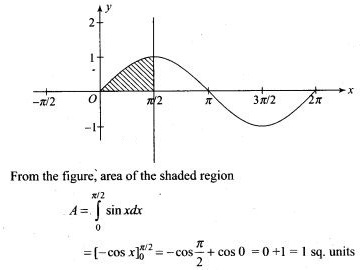
\includegraphics[width=8cm]{sin.jpg}
    \caption{Exact Value of the definite integral.}
    \label{fig:sin}
    \end{figure}
    We plot the absolute error versus length of a subinterval ($\Delta x$) for each of the four methods discussed earlier in this chapter. We also try plotting the semi-log and log-log plot of the same to see if the plots give us a better insight into the nature of differences between the methods. We then apply linear regression to each of the plots.\\
    We then comment on the order of accuracy, accuracy of each method and then present the concluding remark of the report.
    
\chapter{Results}
This chapter takes us through the results obtained by executing the various codes discussed earlier for the 4 methods. Results include the plots for $|E|$ vs $N$, $log(|E|)$ vs $h$, $log(|E|)$ vs $log(h)$, $|E|$ vs $h$ and comparison of the execution time for each root finding algorithm.\\
Note: The execution times stated here are majorly dependent on the way I have implemented the maths into the python code. However, it gives a brief sense of the relative efficiencies of the methods.
\section{Plots}
Here, we present the plots obtained from codes for various methods for Numerical Quadrature. Figure~\ref{fig:Plot1}, \ref{fig:Plot2} , \ref{fig:Plot3} \ref{fig:Plot4} are the plots for the Left , Right , Midpoint and Trapezoidal Methods, implemented for equation \ref{eqn:integral}, obtained by varying the number of subintervals from 10 to 1000, using a step size of 10.\\
Figures \ref{fig:normal}, \ref{fig:semilog} and \ref{fig:loglog} show the $|E|$ vs $h$, $log(|E|)$ vs $h$ and $log(|E|)$ vs $log(h)$ for all the methods, each in one plot- : to ease visual distinction. Also, linear regression is performed in each set raw data obtained.\\
In figures \ref{fig:semilog} and \ref{fig:loglog}, the plots for Left(Blue) and Right(Orange) Endpoint methods overlap. For better scaled up plots, please visit \href{https://github.com/YashIITM/Numerical-Quadrature}{github}.


\begin{figure}[!h]
\centering
\begin{subfigure}{.55\textwidth}
  \centering
  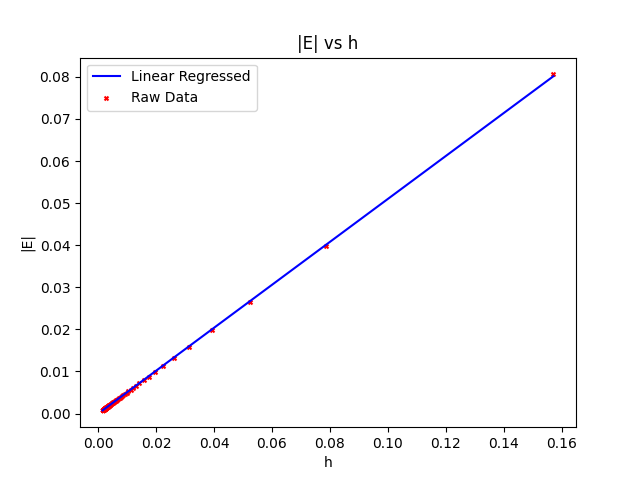
\includegraphics[width=.95\linewidth]{LM1.png}
  \caption{$|E|$ vs $h$}
\end{subfigure}%
\begin{subfigure}{.55\textwidth}
  \centering
  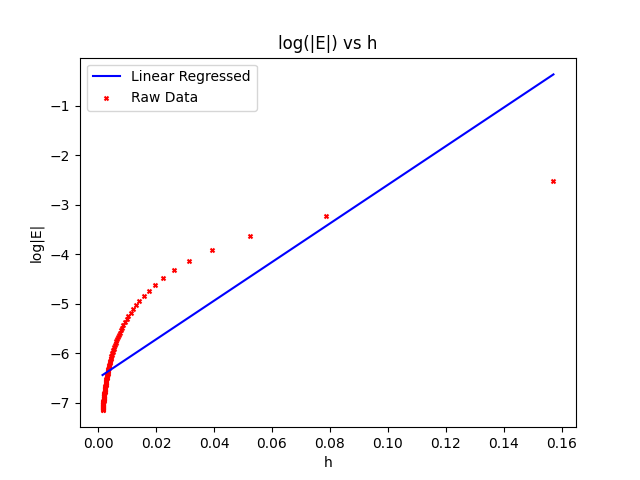
\includegraphics[width=.95\linewidth]{LM2.png}
  \caption{$log(|E|)$ vs $h$}
\end{subfigure}
\begin{subfigure}{.55\textwidth}
  \centering
  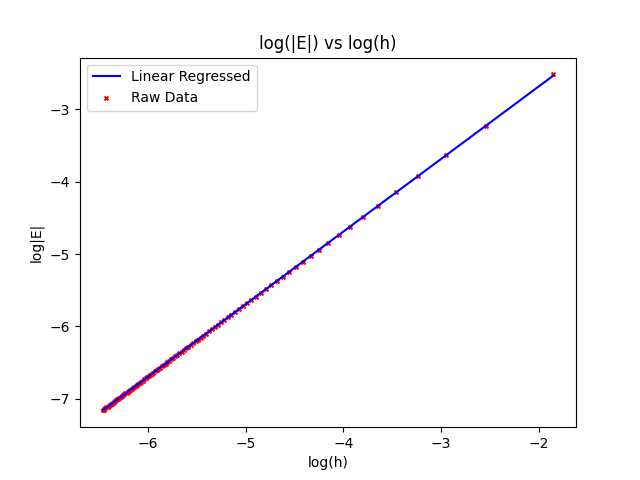
\includegraphics[width=.95\linewidth]{LM3.png}
  \caption{$log(|E|)$ vs $log(h)$}
\end{subfigure}
\caption{Plots for \textbf{Left-Endpoint Method}.}
\label{fig:Plot1}
\end{figure}
\begin{figure}[!h]
\centering
\begin{subfigure}{.55\textwidth}
  \centering
  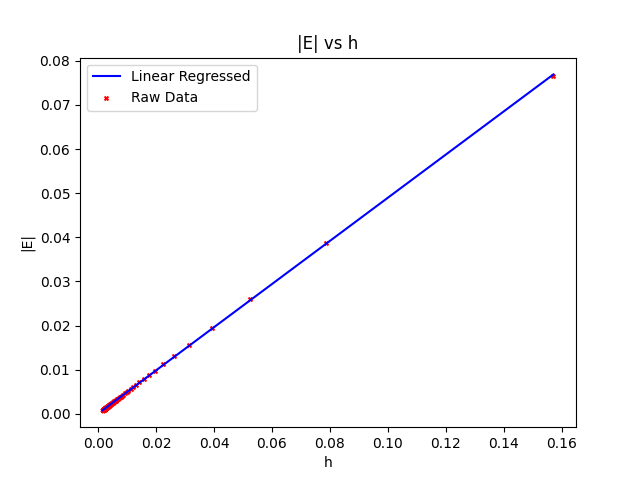
\includegraphics[width=.95\linewidth]{RM1.png}
  \caption{$|E|$ vs $h$}
\end{subfigure}%
\begin{subfigure}{.55\textwidth}
  \centering
  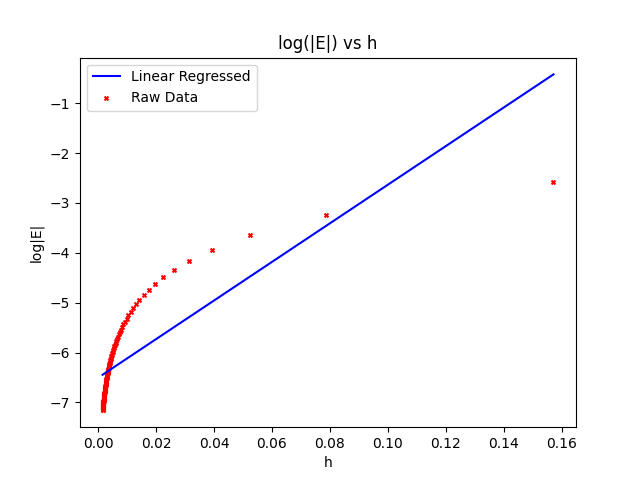
\includegraphics[width=.95\linewidth]{RM2.png}
  \caption{$log(|E|)$ vs $h$}
\end{subfigure}
\begin{subfigure}{.55\textwidth}
  \centering
  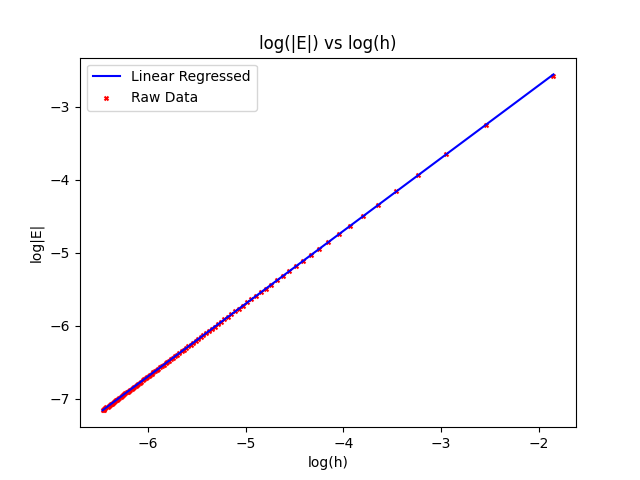
\includegraphics[width=.95\linewidth]{RM3.png}
  \caption{$log(|E|)$ vs $log(h)$}
\end{subfigure}
\caption{Plots for \textbf{Right-Endpoint Method}.}
\label{fig:Plot2}
\end{figure}
\begin{figure}[h]
\centering
\begin{subfigure}{.55\textwidth}
  \centering
  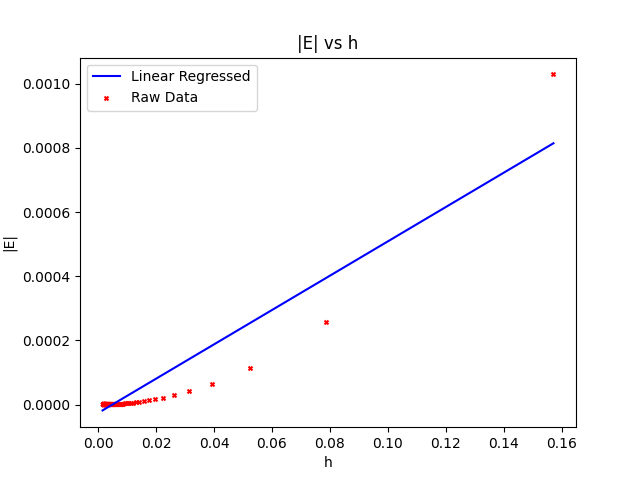
\includegraphics[width=.95\linewidth]{MpM1.png}
  \caption{$|E|$ vs $h$}
\end{subfigure}%
\begin{subfigure}{.55\textwidth}
  \centering
  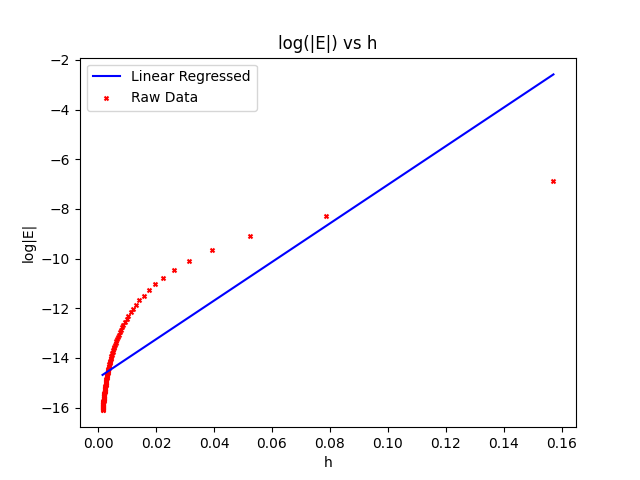
\includegraphics[width=.95\linewidth]{MpM2.png}
  \caption{$log(|E|)$ vs $h$}
\end{subfigure}
\begin{subfigure}{.55\textwidth}
  \centering
  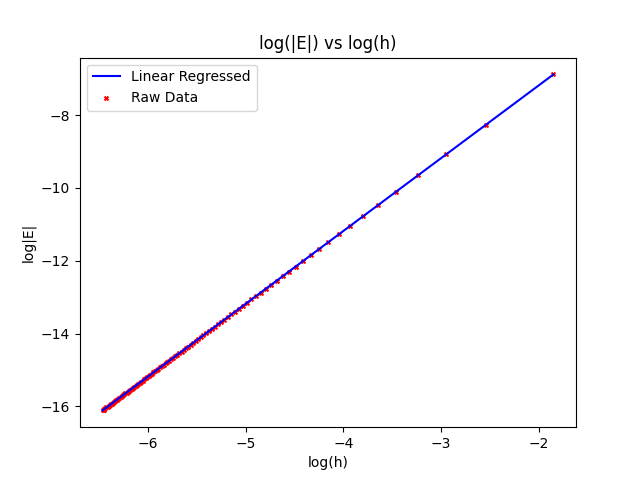
\includegraphics[width=.95\linewidth]{MpM3.png}
  \caption{$log(|E|)$ vs $log(h)$}
\end{subfigure}
\caption{Plots for \textbf{Midpoint Method}.}
\label{fig:Plot3}
\end{figure}
\begin{figure}[!h]
\centering
\begin{subfigure}{.55\textwidth}
  \centering
  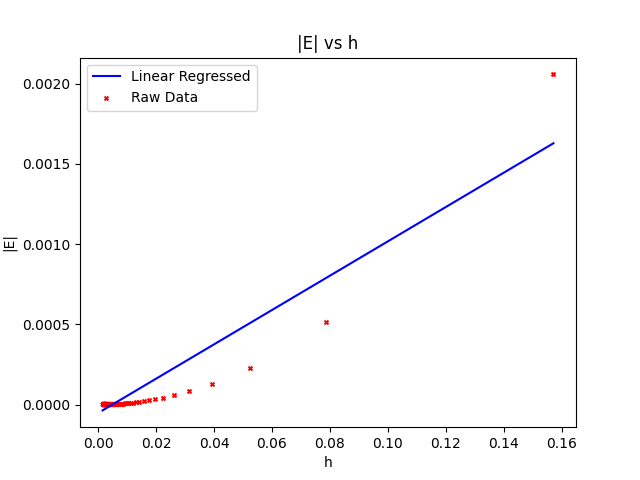
\includegraphics[width=.95\linewidth]{TM1.png}
  \caption{$|E|$ vs $h$}
\end{subfigure}%
\begin{subfigure}{.55\textwidth}
  \centering
  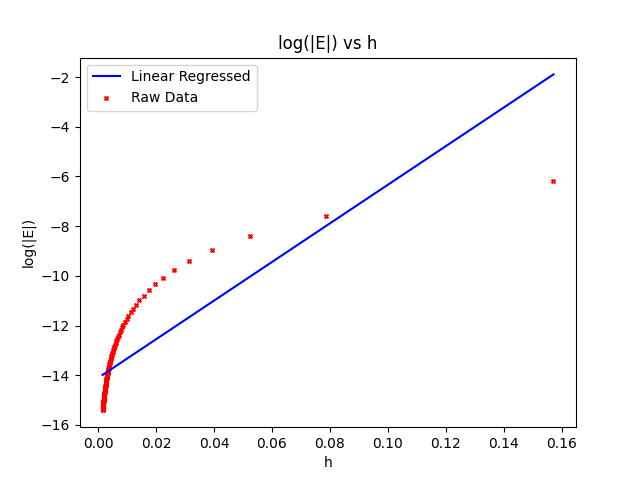
\includegraphics[width=.95\linewidth]{TM2.png}
  \caption{$log(|E|)$ vs $h$}
\end{subfigure}
\begin{subfigure}{.55\textwidth}
  \centering
  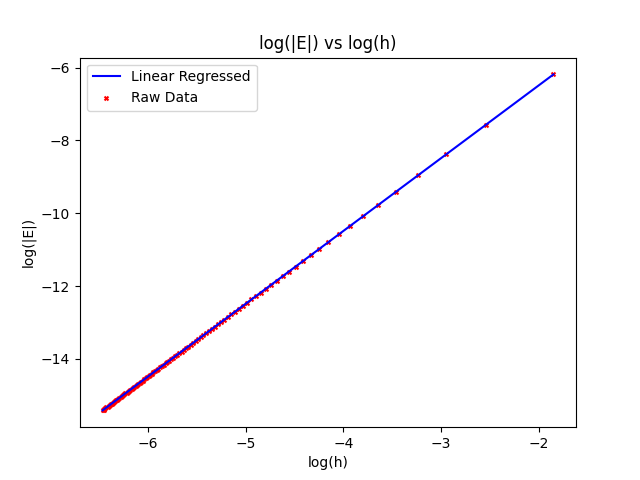
\includegraphics[width=.95\linewidth]{TM3.png}
  \caption{$log(|E|)$ vs $log(h)$}
\end{subfigure}
\caption{Plots for \textbf{Trapezoid Method}.}
\label{fig:Plot4}
\end{figure}


\begin{figure}[!h]
    \centering
    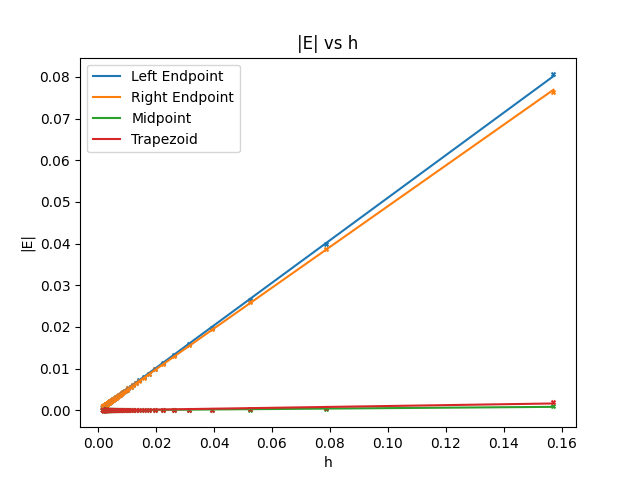
\includegraphics[width=10cm]{normal.png}
    \caption{$|E|$ vs $h$ for all methods.}
    \label{fig:normal}
    \end{figure}
\begin{figure}[!h]
    \centering
    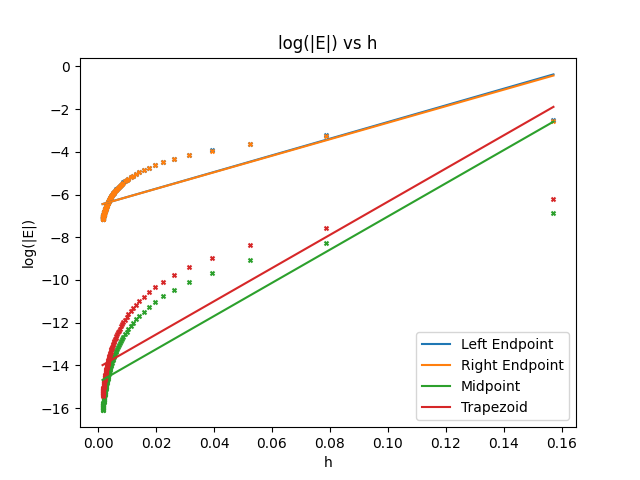
\includegraphics[width=10cm]{semilog.png}
    \caption{$log(|E|)$ vs $h$ for all methods.}
    \label{fig:semilog}
    \end{figure}
\begin{figure}[!h]
    \centering
    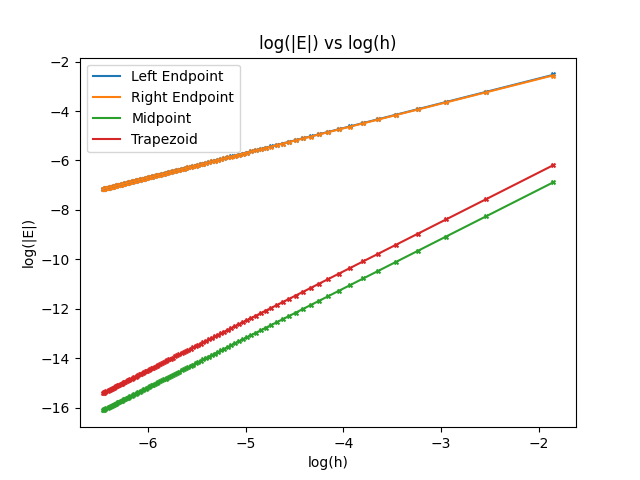
\includegraphics[width=10cm]{loglog.png}
    \caption{$log(|E|)$ vs $log(h)$ for all methods.}
    \label{fig:loglog}
    \end{figure}
\section{Order of Accuracy}
The order of accuracy of the various methods are discussed here. The term 'Order of Accuracy' was defined earlier in Chapter -1.4.\\
We mention the order of accuracy of the methods here as per the definition provided earlier.\\
\textbf{Trapezoid Method: }\\
The order of accuracy is 2 as 
\begin{equation}
        \abs{ \int_{a}^{b} f(x)\,dx\  - A_{trap}} \leq \frac{M_{2}(b-a)^{3}}{12n^{2}}
    \end{equation}
\textbf{Midpoint Method: }\\
The order of accuracy is 2 as
\begin{equation}
        \abs{ \int_{a}^{b} f(x)\,dx\  - M_{n}} \leq \frac{M_{2}(b-a)^{3}}{24n^{2}}
    \end{equation}
\textbf{Right and Left Endpoint Method: }\\
The order of accuracy is 1 as
 \begin{equation}
        \abs{ \int_{a}^{b} f(x)\,dx\  - R_{n}} \leq \frac{M_{1}(b-a)^{2}}{2n}
    \end{equation}
    
    
\chapter{Conclusion}
In this report, we discussed and presented the various methods for Numerical Quadrature, explain the numerical implementation in Python and then apply the results for a simple definite integral of $sin(x)$ in $[0,\frac{\pi}{2}]$.\\ We used Linear Regression to produce a linear plot using the raw data generated using the codes presented in Chapter-2.\\
We also discussed the order of accuracy for each of the methods. Following plot, figure ~\ref{fig:last} shows the plot for $|E| vs N$ (Absolute Error versus No of sub-intervals). The plot (linear regressed) for Trapezoid(red) and Midpoint(green), and Left(blue) and Right(orange) Methods overlap. 

\begin{figure}[h]
    \centering
    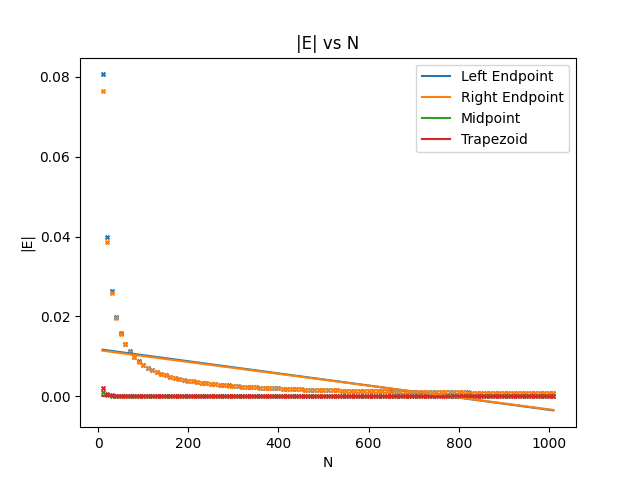
\includegraphics[width=10cm]{last.png}
    \caption{$|E|$ vs $N$ for all methods - 100 data pints.}
    \label{fig:last}
    \end{figure}

 \begin{figure}[h]
    \centering
    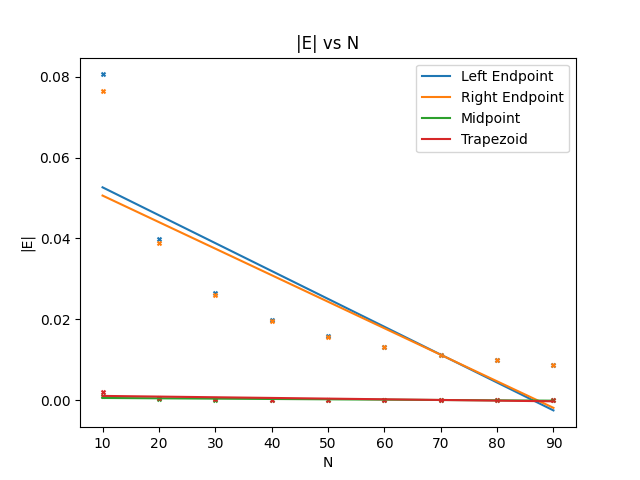
\includegraphics[width=10cm]{last2.png}
    \caption{$|E|$ vs $N$ for all methods - 10 data points.}
    \label{fig:last}
    \end{figure}

For a better scaled up figure, please visit \href{https://github.com/YashIITM/Numerical-Quadrature}{github}.\\
To comment on the accuracy of the 4 methods, consider figure ~\ref{fig:last2} where the same process is repeated for 10 data points, starting from 10 sub-intervals to 100 sub-intervals.
Accuracy is high when $|E|$ is low. From this figure, it's apparent that the accuracy for low number of sub-intervals is higher in Midpoint and Trapezoid Methods when compared to Left and Right Endpoint Methods. However, there exists an N such that past that number of sub-intervals
the accuracy of Left and Right Endpoint Methods are higher!(\ref{fig:last})\\
For the detailed codes in Python, please visit \href{https://github.com/YashIITM/Numerical-Quadrature}{github}.
    \printbibliography

    \appendix

  
\end{document}
